% Bluestift Manifesto — blueprint + research notebook
% Compile on Overleaf: pdfLaTeX + BibTeX
% (upload the whole manuscript/ folder, plus bluestift-mark.png
%  copied from public/bluestift-mark.png in the repo)
\documentclass[11pt,a4paper]{article}
\usepackage[utf8]{inputenc}
\usepackage[T1]{fontenc}
\usepackage{lmodern}
\usepackage[margin=2.6cm,headheight=28pt]{geometry}
\usepackage{hyperref}
\usepackage{graphicx}
\usepackage{booktabs}
\usepackage{enumitem}
\usepackage{xcolor}
\usepackage{fancyhdr}
\usepackage{tikz}
\usetikzlibrary{positioning,shapes.geometric,arrows.meta,calc}
\hypersetup{colorlinks=true,linkcolor=blue!40!black,citecolor=blue!40!black,urlcolor=blue!40!black}
\setlength{\parskip}{0.5em}
% Brand colours — the landing header's two-tone wordmark, light theme
% (components/site/theme.ts: wordmarkA/wordmarkB; Navbar.tsx: weight 800,
% tracking -0.02em, family var(--font-display) -> Space Grotesk).
\definecolor{wordmarkA}{HTML}{173D8A}
\definecolor{wordmarkB}{HTML}{2F7FE0}
% Product mastery thresholds (masteryColor in components/school-admin.tsx).
\definecolor{masteryGood}{HTML}{22C55E}
\definecolor{masteryMid}{HTML}{F59E0B}
\definecolor{masteryLow}{HTML}{EF4444}
\definecolor{masteryNone}{HTML}{6B7794}
% Actor accents from the landing Kernel band (KernelDiagrams.tsx palette, light).
\definecolor{actorLearner}{HTML}{6D28D9}
\definecolor{actorSurface}{HTML}{1D4ED8}
\definecolor{actorKernel}{HTML}{047857}
\definecolor{actorTeacher}{HTML}{B45309}
\newcommand{\bluestiftword}{{\sffamily\bfseries\large\textcolor{wordmarkA}{Blue}\textcolor{wordmarkB}{Stift}}}
\pagestyle{fancy}
\fancyhf{}
\fancyhead[L]{%
  \IfFileExists{bluestift-mark.png}{\includegraphics[height=9mm]{bluestift-mark.png}\hspace{2mm}}{}%
  \bluestiftword%
}
\fancyhead[R]{{\sffamily\small\textcolor{wordmarkA}{Bluestift Manifesto}}}
\fancyfoot[C]{{\sffamily\footnotesize\thepage}}
\renewcommand{\headrulewidth}{0.4pt}
\fancypagestyle{plain}{%
  \fancyhf{}%
  \fancyhead[L]{%
    \IfFileExists{bluestift-mark.png}{\includegraphics[height=9mm]{bluestift-mark.png}\hspace{2mm}}{}%
    \bluestiftword%
  }%
  \fancyhead[R]{{\sffamily\small\textcolor{wordmarkA}{Bluestift Manifesto}}}%
  \fancyfoot[C]{{\sffamily\footnotesize\thepage}}%
  \renewcommand{\headrulewidth}{0.4pt}%
}
% Each major section starts on its own page.
\let\oldsection\section
\renewcommand{\section}{\clearpage\oldsection}
\newcommand{\authorname}{The Bluestift Team}
% TODO(tests): filled from `npm test` (vitest) run of 6 Nov 2026
\newcommand{\vitestcount}{1306}
\newcommand{\vitestfiles}{104}

% PDF metadata only --- the visual cover is built by hand below.
\title{Bluestift: A Shared AI Tutor for the Dissociated Classroom (product blueprint and research notebook)}
\author{\authorname}
\date{November 2026}

\begin{document}
\begin{titlepage}
\begin{center}
\vspace*{4mm}
{\LARGE\bfseries A Shared AI Tutor for the Dissociated Classroom\par}
\vspace{3mm}
{\large A product blueprint and research notebook\par}
\vspace{6mm}
{\large\authorname\par}
\vspace{1mm}
{\small\texttt{contact@thebluestift.com}\par}
\end{center}
\vfill
\begin{center}
\IfFileExists{bluestift-mark.png}{\raisebox{-7mm}{\includegraphics[height=24mm]{bluestift-mark.png}}\hspace{2mm}}{}%
{\fontsize{40}{40}\selectfont\sffamily\bfseries\textcolor{wordmarkA}{Blue}\textcolor{wordmarkB}{Stift}\par}
\end{center}
\vfill
\begin{abstract}
Education is in a dual crisis of access and outcomes: 272~million children and
youth are out of school~\cite{uis-scorecard-2025}, roughly six in ten children
cannot read a simple text by age ten~\cite{wb-cta-2025}, and the world will be
short 44~million teachers by 2030~\cite{unesco-teachers-2024}. Meanwhile,
generative AI has put a private tutor in every student's pocket and a private
assistant on every teacher's desk --- and the two do not talk to each other.
Homework, the last lossy telemetry about how a student thinks, now comes back
laundered: teachers know less about their students than in 2019. We call this
\emph{dissociation}, and Bluestift is the AI the two sides share: a personal,
high-performing tutor for every learner, wired into a collaborative,
safe and stimulating environment. This document is both the product blueprint
(pre-launch; zero users at the time of writing) and the open research
notebook: what we built, what we measured, what we honestly do not know yet,
and the experiments that will decide.
\end{abstract}
\vspace{6mm}
\begin{center}
{\small November 2026 \quad \texttt{thebluestift.com}\par}
\end{center}
\vfill
\end{titlepage}

\tableofcontents
\newpage

%====================================================================
\section{Introduction}
%====================================================================

Two facts define this document. First, we believe the central
educational problem of the late 2020s is not content scarcity but
\emph{dissociation}: teachers and students share only a syllabus while each
side now works privately with its own AI. Second, Bluestift is pre-launch:
the product is built and demoable, and every claim about learning outcomes in
this text is either cited from third-party research or explicitly labelled as
projection. Section~\ref{sec:results} states what we have measured (an
automated test suite of \vitestcount{} tests) and what we have not (anything
involving real learners).

The product thesis, as pitched on video: \emph{put a personal, ultra-performing
tutor in every student's pocket, and connect all of it inside a collaborative,
safe, stimulating --- even exciting --- environment for everyone.} The tutor is
Raya; the shared layer is the Kernel (per-concept cognitive state); the
institutional surface is Bluestift for Schools. The guardrail that holds the
whole design together: \emph{understanding, not surveillance} --- teachers see
secured and shaky concepts, never transcripts.

%====================================================================
\section{Education in the world: the numbers}
\label{sec:numbers}
%====================================================================

\paragraph{Access.} UNESCO's 2025 SDG~4 Scorecard puts the global out-of-school
population at \textbf{272~million} children and youth (2023 data), 21~million
more than previously estimated~\cite{uis-scorecard-2025}: 11\% of primary-age
children (78~M), 15\% of lower-secondary adolescents (64~M) and 31\% of
upper-secondary youth. Girls account for 133~million of the total. Countries
are off track by 75~million against their own 2025 benchmarks, against a pledge
to cut the total by 165~million by 2030.

\paragraph{Outcomes.} Access without learning is the deeper crisis. The World
Bank's \emph{learning poverty} indicator --- inability to read and understand a
simple text by age ten --- stands near \textbf{70\%} in the pandemic-adjusted
series still current in 2025, about six in ten children globally, and nine in
ten in Sub-Saharan Africa~\cite{wb-cta-2025}. Pre-pandemic, 53\% of children in
low- and middle-income countries were affected, improving only to a projected
43\% by 2030 at current rates; the lifetime-earnings cost of the lost learning
is estimated at \$21~trillion. Mathematics is systematically under-measured
(the headline indicator covers reading only), so the true numeracy crisis is
larger than reported.

\paragraph{Measured decline.} PISA~2022 (mathematics focus, results December
2023) recorded an unprecedented fall: the OECD mathematics average dropped to
472, with former top performers sliding for over a decade (Finland: 548 in
2006 to 484)~\cite{oecd-pisa2022}. The 2024 creative-thinking volume averaged
33/60 across the OECD~\cite{oecd-pisa2022-creative}. PISA~2025 (science plus a
new ``Learning in the Digital World'' component) was in the field at the time
of writing, results expected December 2026.

\paragraph{Teachers.} UNESCO's 2024 \emph{Global Report on Teachers} projects a
shortfall of \textbf{44~million} primary and secondary teachers by
2030 --- 15~million in Sub-Saharan Africa alone --- while primary-teacher
attrition nearly doubled from 4.6\% (2015) to 9.1\% (2022)~\cite{unesco-teachers-2024}.
Any plan that requires tens of millions of additional human teachers is not a
plan; it is a wish. Tutoring must scale without scaling headcount one-for-one.

%====================================================================
\section{Education in the news: 2025--2026}
\label{sec:news}
%====================================================================

Data describes stocks; the news describes direction. Three currents matter.

\paragraph{1. Students in revolt.} In autumn 2026 France saw its largest
school revolt in years: from September~21, lyc\'eens blockaded hundreds of
schools over missing teachers, overcrowded classes, dilapidated buildings and
heat, culminating in 320{,}000 demonstrators on November~1 (government
estimate) and a broader cost-of-living movement. Demands include 15{,}000 new
higher-education places and the abolition of Parcoursup, the university
admissions platform the government now promises to replace by
2028~\cite{ap-france-2026}. Parallel ``Gen~Z'' mobilisations swept Germany,
Italy, Belgium and Albania. The salient fact for builders: the users are angry
at the \emph{conditions} of schooling, not at technology --- a window for tools
that visibly improve daily learning life.

\paragraph{2. The great analogue turn.} Six European countries (Sweden, Finland,
Norway, Denmark, France, Italy) moved in 2025--2026 to restrict screens,
phones and --- in Norway's case --- AI in schools~\cite{wef-edtech-2026}.
France, which banned phones in 2018, extended the ban through lyc\'ee (to age
18) at the 2026 rentr\'ee; Sweden will collect phones at the door from autumn
2026 (ages 7--16) and has poured over 2~billion kronor into printed textbooks.
UNESCO estimated ~40\% of world education systems would restrict phones by end
2024, and 35 US states had limits for 2025--26. The lesson is not ``ban
technology'' but \emph{deliberate} digital use: the classroom screen must earn
its place every minute.

\paragraph{3. AI: from bans to bargaining.} The arc runs from prohibition to
negotiated adoption. Sciences~Po banned ChatGPT in January 2023 (France's
first)~\cite{sciencespo-2023}; France's June~2025 national \emph{Framework for
AI Use in Education} instead graduated access (concepts only in primary,
teacher-supervised use from \emph{quatri\`eme}) and explicitly warned teachers
\emph{against} AI-content detectors as unreliable~\cite{france-men-ai-2025}.
Across the Atlantic, the American Federation of Teachers and United Federation
of Teachers signed a legally enforceable AI safety-and-privacy standard with
Microsoft in September 2026 (effective November~1; no training on
student/educator data)~\cite{aft-microsoft-2026}, months after AFT's president
demanded screen bans pre-K--2, no AI in elementary classrooms and no companion
chatbots under 16. The regulatory floor is now set: UNESCO's 2023 guidance
(age~13 minimum, human oversight, no fully automated high-stakes
decisions)~\cite{unesco-ai-2023} and the EU AI Act (education as high-risk use,
emotion recognition banned in schools, AI-literacy duties since February
2025)~\cite{eu-aiact-2024}. Bluestift's compliance posture
(Section~\ref{sec:policy}) is designed against exactly this floor.

%====================================================================
\section{AI and learning: what the research says}
\label{sec:research}
%====================================================================

The oldest result is still the load-bearing one. Bloom (1984) showed that
one-to-one tutored students perform \textbf{two standard deviations} above
classroom-taught peers --- the average tutored student exceeds 98\% of the
control group --- and posed the ``2~sigma problem'': find group methods as
effective as individual tutoring~\cite{bloom-1984}. Forty years of edtech
mostly failed it. Large language models are the first technology that plausibly
passes, and 2025 produced the first serious evidence.

\paragraph{Human-in-the-loop beats human-only (Eedi + Google DeepMind, summer
2025).} Across five UK secondary classrooms (165 students, 17 tutors), core
instruction delivered by LearnLM under expert-tutor supervision matched the
human gold standard at fixing mistakes immediately (93.0\% vs 91.2\%) and
resolving underlying misconceptions (95.4\% vs 94.9\%), then \emph{doubled} the
human tutor's impact on knowledge transfer to new problems (+10.0~pp vs
+4.5~pp over hints)~\cite{eedi-learnlm-2025}. This builds on Eedi's 2023--24
RCT (n=2{,}901): +2 to +4 months of additional maths progress over a school
year. A US RCT with Imagine Learning is scheduled for 2026. Two details matter
for Bluestift: tutors described the AI as ``cognitive offload'' letting them
hold several one-on-one-quality threads at once, and the winning configuration
was \emph{human-in-the-loop} --- exactly our teacher-in-the-loop design
(Section~\ref{sec:product}).

\paragraph{Frontier models tutor in low-resource settings (Nigeria RCT, 2025).}
Six weeks of GPT-4-powered Copilot tutoring for first-year senior-secondary
English learners yielded \textbf{+0.31~SD} on aligned assessments ---
a large effect for a short, cheap intervention, in precisely the
teacher-scarce context of Section~\ref{sec:numbers}~\cite{nigeria-2025}.

\paragraph{Our positioning.} (i) Tutoring works; the 2-sigma prize is real and
now partially claimed. (ii) The scalable form is human-AI teams, not
autonomous agents --- teachers direct, AI executes, humans verify. (iii)
Evidence is young, mostly short-horizon and English-maths-heavy; long-horizon
retention, transfer across subjects, and low-connectivity deployment are open
(research items R1--R3, Section~\ref{sec:notebook}). We cite no vendor market
sizing in this document: analyst estimates for ``AI tutoring markets'' vary by
an order of magnitude and none is peer-reviewed.

%====================================================================
\section{Theoretical foundations: the corpus behind the Kernel}
\label{sec:foundations}
%====================================================================

\paragraph{Why a corpus.} Before the Kernel was an API, it was a reading
list. The team assembled a 23-document corpus --- knowledge tracing,
cognitive psychology, tutoring systems, AI safety, knowledge graphs --- and
distilled it into an operational synthesis in four layers (tracing algorithm,
tutor interaction, curricular representation, institutional deployment), each
paper mapped to the product decision it justifies. Figure~\ref{fig:chain}
shows the causal spine; the paragraphs below walk it layer by layer. All
citations are drawn from our internal research notes, with primary venues
named so that every claim is checkable against the original.

\paragraph{Tracing lineage: from BKT to Responsible-DKT.} Corbett and
Anderson's Bayesian Knowledge Tracing~\cite{corbett-1995} is the root: a
two-state model with four parameters per skill (initial knowledge, learning
rate, guess, slip), a per-skill fit (correlation 0.47 $\to$ 0.85 once
parameters vary by rule), and the mastery criterion the product still uses,
$p(L) \geq 0.95$. Piech et al.'s Deep Knowledge Tracing~\cite{piech-2015}
replaced binary states with a continuous latent vector and gained +25\% AUC
on Khan and ASSISTments data --- but needs large datasets and reads as a
black box. Hooshyar et al.'s Responsible-DKT~\cite{hooshyar-2026} is the
synthesis the Kernel targets: symbolic rules (\texttt{mastered} /
\texttt{not\_mastered}) injected into a neural backbone reach AUC 0.90, hold
above 0.80 on 10\% of the training data, and show that error patterns
outweigh success patterns in updates --- so Bluestift weights errors above
successes. Three refinements complete the lineage: Baker et
al.~\cite{das-baker-2021} show the neural advantage is front-loaded at cold
start (BKT at chance, 0.49, against 0.65 neural on attempt one, converging by
attempt three), hence the cold/warm operating modes; Yudelson et
al.~\cite{yudelson-2013} prove the student-specific parameter worth learning
is the learning rate $p(T)$ (dimension V), not prior knowledge; Ostrow et
al.~\cite{ostrow-2015} replace binary correctness with continuous partial
credit (338k logs), hence $\Delta K = f(\text{partial credit}, \text{KC
difficulty})$.

\paragraph{Tutoring interaction: guardrails are structural.} Bastani et
al.~\cite{bastani-2024} ran the RCT the whole design hinges on:
$\sim$1{,}000 high-schoolers, GPT without guardrails lifting practice scores
+48\% while \emph{cutting} exam scores $-17\%$ --- performance up, learning
destroyed. Raya's hard rules exist because of that number. Sweller's
cognitive load theory~\cite{sweller-1988} explains the mechanism
(goal-directed solving consumes the working memory that schema acquisition
needs) and prescribes the sequence the tutor follows: worked examples, then
goal-free problems (4--6x fewer errors than conventional drill),
conventional exercises last and for measurement only. Lippert and Graesser's
conversational-tutor review~\cite{lippert-2020} supplies the EMT ladder
(PUMP $\to$ HINT $\to$ ASSERTION $\to$ SUMMARY, AutoTutor +0.80$\sigma$),
vicarious demonstration when K is near zero, and productive confusion only
once K and P are solid. Marsh and Rajaram~\cite{marsh-2019} add three
constraints from the psychology of cognition: mere availability of help
degrades encoding (hint-on-demand, never announce help early), retrieval
attempts beat re-reading even when they fail (a pump is mandatory before any
hint, after Roediger \& Karpicke via \cite{marsh-2019}), and assisted
attempts inflate self-assessed mastery (the Kernel down-weights them). Dweck~\cite{dweck-2006}
makes M a dynamic state variable --- process praise only, deflect errors onto
the content when M is low, eight sessions suffice to reverse declining
trajectories, and stereotype threat dissolves under growth mindset, a
protection variable for the target population --- and Luckin~\cite{luckin-2018}
defines what M contains beyond K: metacognition, meta-emotion,
metacontextual awareness, self-efficacy (the strongest non-cognitive
predictor of PISA maths scores).

\paragraph{Representation: two graphs.} Abu-Rasheed et
al.~\cite{aburasheed-2025} fix the unit of analysis at the sub-topic (F1
$\geq$ 0.94 on automated extraction), motivate the split between a dynamic
learner-state graph and a semi-static curricular graph, and add
\texttt{semantically\_equivalent\_to} edges so mastery transfers across
courses instead of restarting from zero. Bian's survey~\cite{bian-2025}
formalises the construction pipeline --- schema-based ontology anchored in
the national curriculum, LLM extraction, LLM-guided fusion --- and points
retrieval at GraphRAG over the graph rather than flat vector search, the only
shape that answers multi-hop prerequisite queries. Liu et
al.~\cite{lpitutor-2025} justify the dual-layer prompt empirically (LLM alone
0.72, RAG alone 0.88 but pedagogically inert, layered 0.94): retrieval
without injected learner state is factually right and pedagogically dead.
Wang et al.~\cite{genmentor-2025} contribute the (status, preferences,
behaviour) learner profile, a simulator to bootstrap cold start, and
goal-to-skill decomposition by chain-of-thought (recall 0.48 zero-shot, good
enough to seed the graph at MVP).

\paragraph{Safety and deployment.} Amodei et al.~\cite{amodei-2016} frame
three Kernel guarantees: Goodhart's law (measure what the student cannot get
by proxy --- response time, error trajectory, unaided behaviour), silent
failure under distributional shift (every tracing model is calibrated on
North-American data, so OOD detection plus local recalibration ship from day
one), and scalable oversight (teachers validate a sample of inferences, the
model extrapolates). The Digital Education Council's 2024 student survey (86\%
already use AI academically, 80\% dissatisfied with their institution's
integration, 5\% know its AI guidelines~\cite{dec-survey-2024}) sizes the
institutional gap the product sells into. Two confirmations close the corpus:
Uddin et al.'s 199-paper systematic review~\cite{uddin-2026} documents
training-data bias and excessive dependency at industrial scale, and
SkillEvolBench~\cite{skillevol-2026} validates selective state updates (not
every interaction deserves one), a short episodic window alongside the
abstract profile, and held-out validation to catch false mastery.

\begin{figure}[h]
\centering
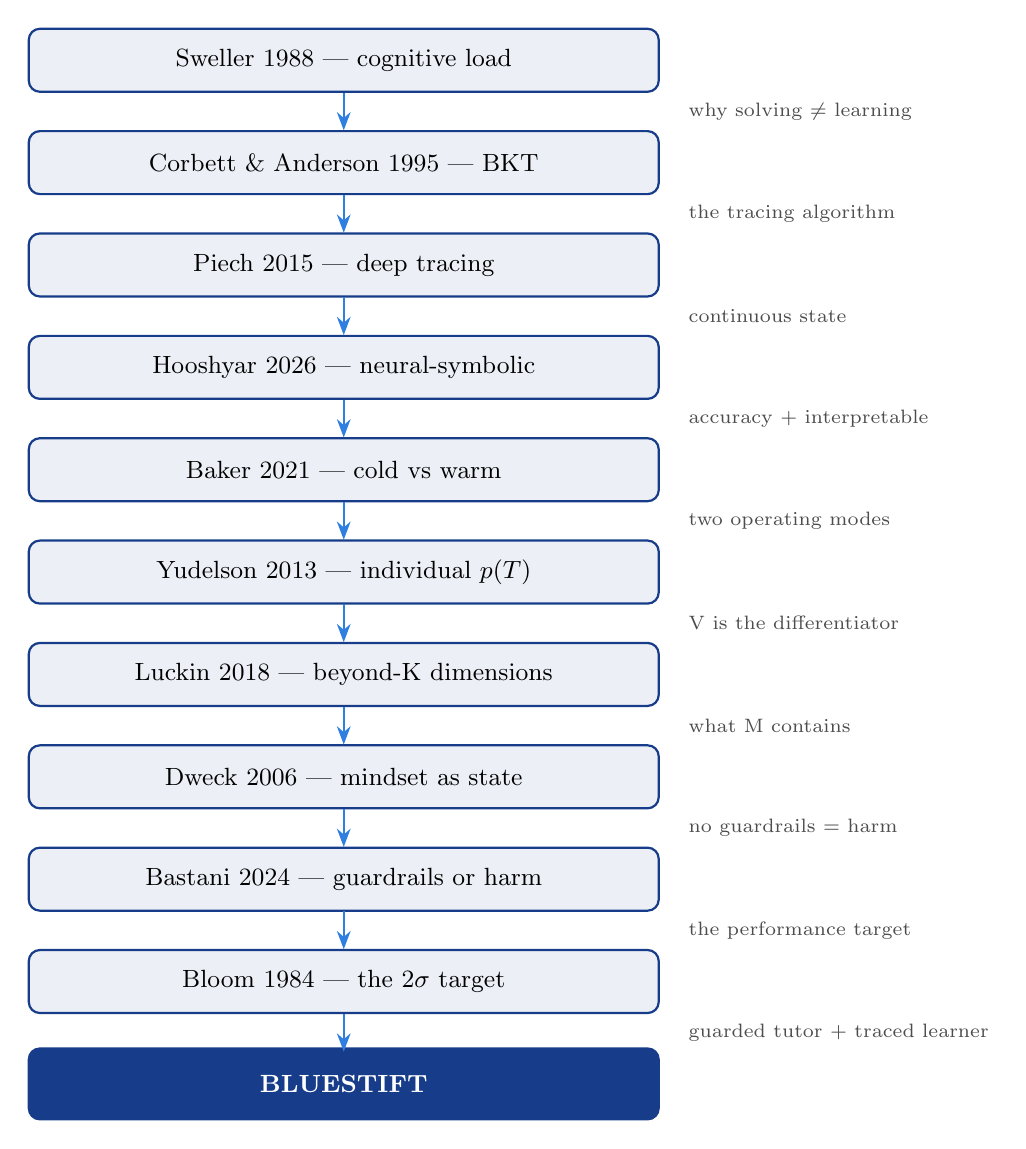
\begin{tikzpicture}[>=Stealth, thick,
  link/.style={draw=wordmarkA, fill=wordmarkA!8, rounded corners,
    minimum width=80mm, minimum height=8mm, align=center, font=\small},
  end/.style={draw=wordmarkA, fill=wordmarkA, rounded corners,
    minimum width=80mm, minimum height=9mm, align=center,
    font=\small\bfseries, text=white}]
\foreach \y/\t in {13/Sweller 1988 --- cognitive load, 11.7/Corbett \& Anderson 1995 --- BKT, 10.4/Piech 2015 --- deep tracing, 9.1/Hooshyar 2026 --- neural-symbolic, 7.8/Baker 2021 --- cold vs warm, 6.5/Yudelson 2013 --- individual $p(T)$, 5.2/Luckin 2018 --- beyond-K dimensions, 3.9/Dweck 2006 --- mindset as state, 2.6/Bastani 2024 --- guardrails or harm, 1.3/Bloom 1984 --- the 2$\sigma$ target} {
  \node[link] at (5.9,\y) {\t};
}
\node[end] at (5.9,0) {BLUESTIFT};
\foreach \y/\t in {12.35/why solving $\neq$ learning, 11.05/the tracing algorithm, 9.75/continuous state, 8.45/accuracy + interpretable, 7.15/two operating modes, 5.85/V is the differentiator, 4.55/what M contains, 3.25/no guardrails = harm, 1.95/the performance target, 0.65/guarded tutor + traced learner} {
  \draw[->, wordmarkB] (5.9,\y+0.24) -- (5.9,\y-0.24);
  \node[anchor=west, font=\scriptsize, text=black!70] at (10.15,\y) {\t};
}
\end{tikzpicture}
\caption{The causal spine of the corpus: each result answers the question the
previous one left open --- from why solving is not learning (Sweller) to the
performance target (Bloom). Bluestift is the composition: a guarded tutor
over a traced learner.}
\label{fig:chain}
\end{figure}

%====================================================================
\section{The dissociation thesis}
\label{sec:thesis}
%====================================================================

\paragraph{Memory is dead as a pitch.} In 2022, ``an AI tutor that remembers
every student'' was a real edge. By 2026, frontier models ship ~1M-token
context, caching and cross-conversation memory as standard: recall is a
commodity. Bluestift retired the memory pitch in July 2026 and forbids its
return in any wording.

\paragraph{The durable problem.} A teacher and a student share only a syllabus
and fixed objectives: one distributes, the other ingests. Follow-up for
outliers in either direction fails overwhelmingly on the teacher's time
constraint. AI has now \emph{widened} the gap instead of closing it: both
sides hold a private AI, and the two do not communicate. Bluestift is the AI
they \textbf{share} --- teacher directives and class instructions flow down
with an explicit ``From your teacher'' banner; derived per-concept state flows
up into dashboards, focus lists and exam preparation (Figure~\ref{fig:dissociation}).

\paragraph{The acute symptom.} Systemic pain does not open budgets; acute
symptoms do. Ours: \textbf{AI destroyed the last signal channel.} Homework
used to be lossy telemetry about how a student thinks; it now returns
laundered, so a teacher in 2026 knows \emph{less} about each learner than in
2019. Recent, specific, enraging --- a buying trigger, where ``reconnect
teaching and learning'' is only a mission statement.

\paragraph{The guardrail.} \emph{Understanding, not surveillance.} Teachers see
secured and shaky concepts, never transcripts. This is load-bearing, not
decorative: a student who feels read stops admitting confusion, which destroys
the very signal the loop runs on. The same instinct rejected an early
``steer the student'' framing for teacher instructions: the product
\emph{recommends}, transparently, and the student sees the same banner the
teacher wrote.

\begin{figure}[h]
\centering
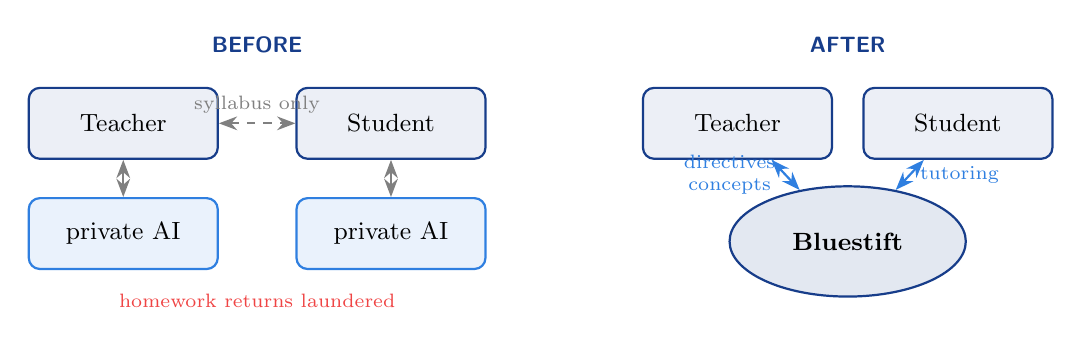
\begin{tikzpicture}[>=Stealth, thick,
  actor/.style={draw=wordmarkA, fill=wordmarkA!8, rounded corners,
    minimum width=24mm, minimum height=9mm, align=center, font=\small},
  ai/.style={draw=wordmarkB, fill=wordmarkB!10, rounded corners,
    minimum width=24mm, minimum height=9mm, align=center, font=\small},
  shared/.style={draw=wordmarkA, fill=wordmarkA!12, ellipse,
    minimum width=30mm, minimum height=14mm, align=center,
    font=\small\bfseries}]
% --- before: two private AIs ---
\node[font=\sffamily\bfseries\footnotesize, text=wordmarkA] at (1.7,2.4) {BEFORE};
\node[actor] (t1) at (0,1.4) {Teacher};
\node[actor] (s1) at (3.4,1.4) {Student};
\node[ai] (ta1) at (0,0) {private AI};
\node[ai] (sa1) at (3.4,0) {private AI};
\draw[<->, dashed, gray] (t1) -- node[above, font=\scriptsize] {syllabus only} (s1);
\draw[<->, gray] (t1) -- (ta1);
\draw[<->, gray] (s1) -- (sa1);
\node[font=\scriptsize, text=masteryLow] at (1.7,-0.85) {homework returns laundered};
% --- after: one shared AI ---
\node[font=\sffamily\bfseries\footnotesize, text=wordmarkA] at (9.2,2.4) {AFTER};
\node[actor] (t2) at (7.8,1.4) {Teacher};
\node[actor] (s2) at (10.6,1.4) {Student};
\node[shared] (b) at (9.2,-0.1) {Bluestift};
\draw[<->, wordmarkB] (t2) -- node[left, font=\scriptsize, align=center] {directives\\concepts} (b);
\draw[<->, wordmarkB] (s2) -- node[right, font=\scriptsize] {tutoring} (b);
\end{tikzpicture}
\caption{Dissociation, before and after. Left: each side works privately with
its own AI; teacher and student share only a syllabus, and homework returns
laundered. Right: Bluestift as the shared layer --- teacher directives flow
down under the ``From your teacher'' banner while only per-concept state
(secured and shaky concepts, never transcripts) flows up.}
\label{fig:dissociation}
\end{figure}

\paragraph{Honest risks.} (1) Systemic pain $\neq$ buying trigger --- hence
lead with the symptom. (2) Two-sided cold start: teachers without students get
an empty dashboard; students without a teacher get a worse ChatGPT. (3)
Surveillance framing can eat the pitch (mitigated by the guardrail). (4)
Platform risk: Google owns Classroom, identity and Gemini and could ship the
connective tissue natively. (5) Competition: Khanmigo has teacher visibility
but is locked to Khan content; MagicSchool/Brisk are teacher-side only;
general assistants are student-side only. The pitch is therefore B2B-shaped;
solo Raya is the funnel, not the story. Deliberately, there is no level or
geography targeting --- any level, any subject, anywhere.

%====================================================================
\section{Bluestift today: the product}
\label{sec:product}
%====================================================================

Bluestift is built on Next.js + Supabase + a FastAPI Kernel service.
What follows is \emph{built and wired}, not roadmap.

\paragraph{Raya, the Socratic tutor.} A dual-layer prompt: a static guardrail
layer (never give the answer; EMT escalation PUMP$\to$HINT$\to$ASSERTION$\to$SUMMARY
with an attempt required before any hint; Dweck-style process praise; reply in
the learner's language, reason in English) plus a dynamic layer injecting the
Kernel cognitive vector to set the entry level. LLM stack is Gemini primary
with Groq fallback over plain fetch (no SDK), streamed token-by-token;
voice input runs on Whisper via Groq. The hot path never awaits the Kernel
(60~s profile cache, 6~s fetch timeout): when the Kernel is down, tutoring
degrades gracefully instead of failing. It has been down since July~30, 2026
(Section~\ref{sec:results}) --- which is also a live resilience test.

\paragraph{Funnel: try before signup.} Signed-out visitors get the whole app
rendered locked (``candy store: see, touch, can't eat'') with a working
5-turn stateless guest chat; threads import into the new account at signup.
No captcha on the guest path (abuse contained by turn + per-IP rate limits).

\paragraph{One chat engine.} Student Raya, Raya-for-Schools and rooms' private
channels are literally the same code (\texttt{components/chat/}), driven by a
per-surface \texttt{ChatConfig} adapter (endpoints, capabilities, greeting,
suggestions) --- so the surfaces can never drift apart again.

\paragraph{The Kernel: shared cognitive state.} Every learner carries a
per-concept cognitive vector maintained by the Kernel service: \textbf{K}
(mastery, raw and slip-corrected), \textbf{V} (learning rate), \textbf{P}
(resistance to slipping back, modulated by mindset) and a global \textbf{M}
(mindset reading). Concepts (KCs) are created on the fly from the learner's
own work --- there is no closed-world syllabus list --- and resolution is
cross-subject: a physics request for \texttt{vecteurs} lands on the existing
maths KC instead of forking a duplicate. After each conversation slice,
\texttt{/analyze} returns the diagnosis: \texttt{root\_gap},
\texttt{detection\_path}, a per-concept \texttt{mastery\_map}, a
\texttt{recommended\_path}, pedagogical-safety \texttt{alerts} and a
\texttt{probe} --- the single diagnostic question that would best settle where
the gap is. Graded attempts bypass inference entirely: every challenge,
assignment and quiz answer is sent to \texttt{/update\_concept\_state} with
its real partial-credit score, whether it was assisted, and whether the
question was open (5\% guess rate) or multiple-choice.

\paragraph{How the diagnosis behaves.} The probe plays hot/cold: each answer
moves the Kernel's belief and the next probe goes where uncertainty is
highest, sometimes several floors below the conversation (fractions while the
student works on functions). Raya asks each probe as two open questions,
unassisted and unhinted --- in the Kernel's internal synthetic evaluation
(600 simulated students, gap up to five floors down), that discipline lifts
exact-gap recall after five measures from 42--47\% (single multiple-choice
probe) to 66--75\%. \texttt{mastered} is deliberately strict: K~$\geq$~0.95
plus low personal slip plus mean credit~$\geq$~0.7 on the last three
\emph{unassisted} attempts; a concept merely mentioned, never attempted, is
\texttt{unknown} (``not assessed yet''), never a failure. And the teaching
target is always the \emph{weakest} active concept, never the mean --- a
learner averaging 0.78 with a prerequisite at 0.20 is exactly the case
averaging hides (\texttt{lib/kernel/signals.ts}).

\paragraph{School channel and safety loop.} A school that sets curriculum
layers gets its objectives measured against real mastery (\texttt{met} /
\texttt{at\_risk} / \texttt{overdue} / \texttt{pending} / \texttt{unknown}),
its priorities reordering the \texttt{recommended\_path}, and its rules
injected into Raya's prompt under the ``From your teacher'' banner. Upward,
\texttt{/prerequisite\_gaps} returns missing foundations in teaching order
(deepest first, never re-sorted) with the \texttt{frontier} where the walk
stopped on held concepts; \texttt{/load\_alerts} feeds the dashboard from
persisted safety flags (\texttt{passive\_dependency},
\texttt{false\_mastery}, \texttt{cognitive\_overload},
\texttt{fixed\_mindset}, \texttt{re\_emergence\_error},
\texttt{inconsistency\_high}, \texttt{ood\_distribution}). The dashboard reads
the shared tables directly rather than waking the service per page view, and
an unreachable Kernel fails loud (error state) rather than rendering an empty
``all clear'' --- because on a safety screen, silence is a lie.
Figure~\ref{fig:kernel} shows the loop; Figures~\ref{fig:overview}--\ref{fig:mastery}
show the teacher surface it feeds, as real captures from the demo school.

\begin{figure}[h]
\centering
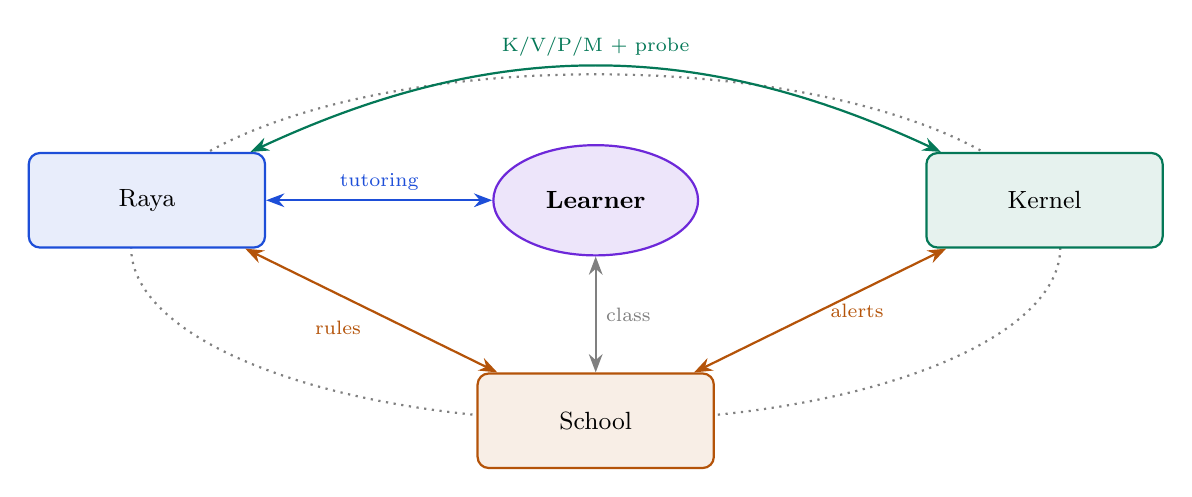
\begin{tikzpicture}[>=Stealth, thick,
  learner/.style={draw=actorLearner, fill=actorLearner!12, ellipse,
    minimum width=26mm, minimum height=14mm, align=center,
    font=\small\bfseries},
  sat/.style={rounded corners, minimum width=30mm, minimum height=12mm,
    align=center, font=\small}]
% orbit
\draw[dotted, gray] (7.9,-1.6) ellipse (5.9cm and 2.2cm);
% actors
\node[learner] (l) at (7.9,-1) {Learner};
\node[sat, draw=actorSurface, fill=actorSurface!10] (r) at (2.2,-1) {Raya};
\node[sat, draw=actorKernel, fill=actorKernel!10] (k) at (13.6,-1) {Kernel};
\node[sat, draw=actorTeacher, fill=actorTeacher!10] (s) at (7.9,-3.8) {School};
% exchanges
\draw[<->, actorSurface] (l) -- node[above, font=\scriptsize] {tutoring} (r);
\draw[<->, actorKernel] (r) to[bend left=25]
  node[above, font=\scriptsize] {K/V/P/M + probe} (k);
\draw[<->, actorTeacher] (k) -- node[right, font=\scriptsize] {alerts} (s);
\draw[<->, actorTeacher] (s) -- node[below left, font=\scriptsize] {rules} (r);
\draw[<->, gray] (s) -- node[right, font=\scriptsize] {class} (l);
\end{tikzpicture}
\caption{The Kernel loop: the learner at the centre, Raya, the Kernel and the
school in orbit, exchanging continuously. Raya tutors from the learner's work;
the Kernel returns per-concept state (K/V/P/M), probes and alerts; the school
sets objectives and rules, and reads mastery --- never transcripts. Actor
colours match the landing page's Kernel band.}
\label{fig:kernel}
\end{figure}

\paragraph{Schools: layer, dashboard, billing.} Onboarding routes teachers and
admins through a school layer (\texttt{/school/enter}): verified school form,
45-day pilot capped at declared headcount ($\geq$100), read-only after expiry.
The teacher workspace spans Overview, Classes, Focus, Prepare, Insights,
Reports, Raya and Settings, with shared follow-up notes, deterministic
exam-prep generation (one JSON call; markdown composed deterministically so doc
and data cannot diverge) and one-attempt assignments with optional deadlines.
Commercial terms are already enforced in code: per-\emph{enrolled}-effectif
billing (never per-active --- charging less when students disengage would be
anti-mission), Student Plus at \$6.99/mo, schools from \$1.50/student/mo,
manual founder activation until a legal entity and Stripe exist.

\begin{figure}[h]
\centering
\includegraphics[width=\textwidth]{"Screenshot 2026-11-07 002039.png"}
\caption{Schools Overview, real capture (Bluestift Demo High, seeded demo
data): KPI tiles, per-class mastery bars, Kernel mastery gauge, alerts and
classes-to-watch panels. No real users at the time of writing.}
\label{fig:overview}
\end{figure}

\begin{figure}[h]
\centering
\includegraphics[width=\textwidth]{"Screenshot 2026-11-07 002247.png"}
\caption{Class roster, real capture (demo data): triage filters (needs
attention / on track / no data) and per-student mastery with drill-down into
each record.}
\label{fig:roster}
\end{figure}

\begin{figure}[h]
\centering
\includegraphics[width=\textwidth]{"Screenshot 2026-11-07 002549.png"}
\caption{Student detail, real capture (demo student): risk badge, mindset
reading, on-demand Raya analysis, and the homework-first report (empty state
shown honestly --- no homework set yet).}
\label{fig:student}
\end{figure}

\begin{figure}[h]
\centering
\includegraphics[width=\textwidth]{"Screenshot 2026-11-07 002659.png"}
\caption{Learning graph, real capture (demo data): per-concept nodes coloured
by mastery (green mastered, amber partial, red gap, grey not started) over
prerequisite edges --- a red foundation node holds back everything below it.}
\label{fig:graph}
\end{figure}

\begin{figure}[h]
\centering
\includegraphics[width=\textwidth]{"Screenshot 2026-11-07 002749.png"}
\caption{Mastery by concept with team-shared follow-up notes, real capture
(demo data): the ranked concept list the teacher acts on, and the running log
shared with the class team.}
\label{fig:mastery}
\end{figure}

\paragraph{Platform facts.} Four locales (EN/FR/ES/DE, $\sim$3{,}100 keys)
covering UI \emph{and} server messages; anonymous-first auth (anon for
learners, verified email required for staff, Turnstile, Resend); a drawn
motion-design explainer film (178~s); public site with landing, research,
survey, contact and feedback. Bill of materials, November 2026: 600 tracked
source files, $\sim$828k words, and a 4{,}165-node product knowledge graph
maintained alongside the repo.

%====================================================================
\section{Method, measures and simulations}
\label{sec:method}
%====================================================================

\paragraph{Automated suite (measured).} \texttt{npm test} (Vitest, run
6~November 2026): \textbf{\vitestcount{} tests across \vitestfiles{} files},
covering pure and safety-critical logic --- name/username rules, the
anonymous-vs-verified auth boundary, email escaping and never-send guards,
fail-open rate limiting, seat-gate arithmetic, licensing gates, i18n key
coverage across all four locales, and theme-contrast/layout uniformity. The
suite is the enforcement arm of the design contracts: several product rules
(school-layer single creation path, locale-key completeness, billing gates)
fail closed in tests before they can fail open in production.

\paragraph{What-if simulation (built, estimates labelled).} Both learners
(\texttt{/profile}) and school admins get grounded what-if projections (``+N
h/week on focus X $\to$ projected mastery''): baseline from the learner's own
Kernel profile (server-overwritten so it cannot drift), projection by a
grounded LLM estimate with confidence badge, stated assumptions, risks and
next steps, persisted per-user with history. Because the Kernel exposes no
simulation endpoint, projections are estimates by construction --- the UI says
so. No outcome claims are made from this feature.

\paragraph{Remediation order is data, not UI.} When a learner is stuck,
\texttt{/prerequisite\_gaps} returns the missing foundations already sorted in
teaching order --- deepest first --- with the frontier of held concepts as
evidence and partial lists labelled partial (Figure~\ref{fig:prereq}). No
client-side re-sorting is allowed (sorting by hops would break the pedagogy);
the app renders the list top to bottom. Values in the figure are illustrative;
the contract and the mastery thresholds are the real ones.

\begin{figure}[h]
\centering
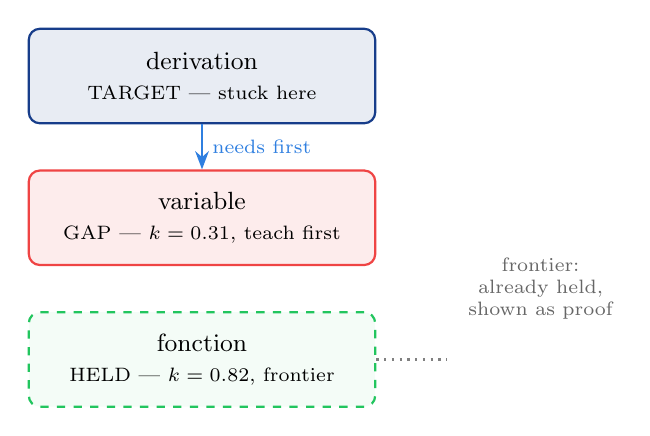
\begin{tikzpicture}[>=Stealth, thick,
  kc/.style={rounded corners, minimum width=44mm, minimum height=12mm,
    align=center, font=\small}]
\node[kc, draw=wordmarkA, fill=wordmarkA!10] (t) at (0,2.8) {derivation\\\scriptsize TARGET --- stuck here};
\node[kc, draw=masteryLow, fill=masteryLow!10] (g) at (0,1.0) {variable\\\scriptsize GAP --- $k=0.31$, teach first};
\node[kc, draw=masteryGood, dashed, fill=masteryGood!5] (f) at (0,-0.8) {fonction\\\scriptsize HELD --- $k=0.82$, frontier};
\draw[->, wordmarkB] (t) -- node[right, font=\scriptsize] {needs first} (g);
\node[font=\scriptsize, text=black!60, align=center] at (4.3,0.1) {frontier:\\already held,\\shown as proof};
\draw[dotted, gray] (f.east) -- (3.1,-0.8);
\end{tikzpicture}
\caption{Remediation order for a stuck concept: gaps arrive in teaching order
(deepest foundation first), with the frontier of held concepts shown as
evidence that a short list is short for a reason. Illustrative values; real
contract (\texttt{/prerequisite\_gaps}) and real mastery thresholds.}
\label{fig:prereq}
\end{figure}

\paragraph{Sizing simulations (projections, assumptions stated).} With zero
users, unit economics are threshold analysis, not results. Table~\ref{tab:thresholds}
states what must hold for the model of Section~\ref{sec:model} to work; each
threshold names the load test or pilot that will measure it. Illustrative
arithmetic only: a 500-student school at \$1.50/student/mo yields \$750/mo
gross; whether LLM spend per tutored student-month fits inside that envelope
depends on turn volume, model mix and caching --- unknown until the first
instrumented pilot (research item R4). We publish the framework now so the
numbers, when they exist, have somewhere to land.

\begin{table}[h]
\centering
\caption{Viability thresholds (projections, not results). Each row names its
deciding experiment.}
\label{tab:thresholds}
\begin{tabular}{@{}lll@{}}
\toprule
Quantity & Must hold & Decided by \\
\midrule
LLM cost / tutored student / month & $< 30\%$ of seat price & R4: instrumented pilot \\
Guest $\to$ signup conversion & $> 5\%$ of triallists & R5: funnel instrumentation \\
Pilot $\to$ paid conversion & $\geq 1$ of first 3 pilots & R6: concierge pilots \\
Knowledge transfer (new problems) & $> 0$ vs hints baseline & R1: Eedi-style trial \\
\bottomrule
\end{tabular}
\end{table}

%====================================================================
\section{Results}
\label{sec:results}
%====================================================================

\paragraph{What passed.} The automated suite is green (\vitestcount{}/\vitestcount{}),
\texttt{tsc}, ESLint and all-route compilation were green at the
finishing pass. That same pass verified that nothing broken is user-reachable: incomplete
surfaces are hidden behind reversible gates, dead billing CTAs read
``temporarily unavailable'', and manual activation (the only live money path)
works end to end.

\paragraph{What is honestly missing.} There are \textbf{no learning-outcome
results}: zero users means zero measurements, and this document will not
extrapolate from demos. The production Kernel has been \textbf{down since
July~30, 2026} (hosting removed; redeploys failed) and has never written a
single output row --- every Kernel-backed feature runs in its designed
degraded mode. Legal pages and the data dossier are mock-grade: a September 2026
code$\leftrightarrow$copy audit aligned copy with code, but no counsel has
reviewed anything, and the under-13 solo-use decision (Section~\ref{sec:policy})
is flagged as the weakest point. Stating this plainly is deliberate: a
blueprint that hides its gaps is a pitch deck, not a research notebook.

%====================================================================
\section{Model and policy}
\label{sec:model}
\label{sec:policy}
%====================================================================

\paragraph{Commercial model.} Until a legal entity and Stripe exist, Bluestift
runs on direct licensing: a school pays the founder, only the founder
activates (schools file licence \emph{requests}). Billing is per enrolled
effectif --- 800 enrolled means 800 paid even if 300 are active --- with the
seat field floored at real headcount so under-contracting is impossible.
Western-calibrated prices (Plus \$6.99 near Khanmigo; schools from
\$1.50/student/mo against \$10--40/student/yr district-AI anchors); Africa
will need a separate purchasing-power price book later, architected as a
region dimension, not a blocker.

\paragraph{Learning and data policy.} Three deliberate decisions: (1) \textbf{no
mastery gate} --- Bloom's threshold is a measurement, not a lock; a tutor that
refuses to answer gets closed. (2) The B2B2C boundary is the linked
\texttt{school\_id}: unlinked, nothing leaves the account; linked, teachers
see mastery, gaps, results and follow-ups --- while Raya conversations stay on
the student's side in \emph{both} cases, and joining a class is disclosed as a
disclosure event. (3) Model training consent: opt-\emph{out} for solo adults,
\emph{never} for minors (age gate runs first and is non-negotiable), explicit
opt-\emph{in} on school-linked accounts (as processor we cannot default a
school's users into our own training).

\paragraph{Compliance status.} The September~6, 2026 audit enforced the age
gate on content-bearing API routes (pages alone were gating), completed the
export bundle, aligned four legal pages in four locales with the code, and
recorded the hard decisions: under-13s may use Raya alone (``a child must be
able to use it even alone''), and \textbf{only an adult pays} (guardian
attestation at checkout, no verification mechanism yet --- flagged for
counsel). Subprocessors, retention, cookie and breach rows are maintained in
\texttt{docs/compliance.md} with the rule that legal copy changes in the same
commit as the code it describes.

%====================================================================
\section{Research notebook: open questions}
\label{sec:notebook}
%====================================================================

Each item names the experiment that closes it. Owners of a result elsewhere in
this document will find its falsifier here.

\begin{description}[leftmargin=!,labelwidth=3em]
\item[R1 Transfer.] Does Raya tutoring transfer to \emph{new} problems (the
Eedi metric, +10~pp human-AI vs +4.5~pp human-only)? \emph{Closes with:}
Eedi-style trial on Bluestift content, hints baseline, transfer endpoint.
\item[R2 Retention.] Do tutored gains persist at 30/90 days? \emph{Closes
with:} delayed post-tests in the first pilot cohort.
\item[R3 Low-connectivity.] What degrades first on 2G/intermittent links ---
streaming, voice, media? \emph{Closes with:} throttled-network test matrix +
outbox/blob retention budgets already specced in \texttt{lib/net}.
\item[R4 Unit cost.] LLM spend per tutored student-month at pilot load, by
model mix and cache hit rate. \emph{Closes with:} instrumented pilot with
per-turn token accounting.
\item[R5 Funnel.] Guest-trial $\to$ signup $\to$ active-learner conversion.
\emph{Closes with:} PostHog funnel (relay live since September 2026) once
traffic exists.
\item[R6 Cold start.] Can one teacher + thirty students bootstrap signal in
week one, or does the dashboard stay empty? \emph{Closes with:} three
concierge pilots, founder on site.
\item[R7 Kernel value.] Does per-concept state measurably beat prompt-only
tutoring (entry-level accuracy, teacher time saved)? \emph{Closes with:}
A/B with Kernel on/off after restoration --- until then, the Kernel is a
hypothesis with an API, not an asset.
\item[R8 Mastery without gates.] Does steering-without-locking keep engagement
\emph{and} progression? \emph{Closes with:} path-adherence vs completion
analysis in pilot data.
\item[R9 Modality frontier.] Text-to-speech overviews, raster diagrams: which
earn their latency and cost? \emph{Closes with:} per-modality A/B on
engagement and transfer; default is \emph{not} to build.
\item[R10 Framing.] Does ``understanding, not surveillance'' hold in real
classrooms, or does teacher visibility chill student honesty? \emph{Closes
with:} confusion-admission rates (help-seeking turns) before/after dashboard
rollout per class.
\end{description}

%====================================================================
\section{Vision and conclusion}
%====================================================================

The end state, stated October 2026: \textbf{annihilate Raya as a standalone
app.} Raya becomes an agent living inside the LMSs and chat tools schools and
students already use; Kernel + Raya become a bridge --- better, a truly social
interface. Sell to schools for volume; build for students, whose engagement
pushes schools to pay more. Schools with no LMS get a visibility space from
Bluestift. The wedge is cross-LMS, cross-year student state plus the no-LMS
long tail; the threats are the LMS vendors' own AIs (Gemini in Classroom for
all ages since August 2026, Canvas+OpenAI, Microsoft's LTI agents) and, on the
novelty axis, Khanmigo. Roadmap rule until then: rank every feature by ``does
it make Raya/Kernel portable into other surfaces''; commodity generators (mind
maps, quizzes) are already free elsewhere and are not the moat.

Bluestift's wager, in one paragraph: the world is short 44~million teachers,
272~million learners are out of school entirely, and the two private AIs on
either side of the classroom have destroyed the last signal channel between
them. Research now shows human-AI tutoring teams matching and amplifying human
tutors. The company being built here is the shared layer --- a personal tutor
in every pocket, connected through a collaborative, safe and stimulating
environment --- instrumented from day one so that every claim in the next
edition of this notebook is a measurement, not a hope.

\clearpage
\bibliographystyle{plain}
\bibliography{references}

\end{document}


